%
% File naaclhlt2012.tex
%

\documentclass[11pt,letterpaper]{article}
\usepackage{vzor/naaclhlt2012}
\usepackage{times}
\usepackage{latexsym}
\setlength\titlebox{6.5cm}    % Expanding the titlebox
\usepackage[utf8]{inputenc}
%\usepackage[utf8]{inputenc}
%\usepackage[russian]{babel}
%\usepackage[T2A]{fontenc}
\usepackage{float/float}
\usepackage{graphicx}
%\usepackage{hyperref}

\title{Unknown words in Statistical Machine Translation between morphologically
rich and poor languages}

%\author{Author 1\\
%	    XYZ Company\\
%	    111 Anywhere Street\\
%	    Mytown, NY 10000, USA\\
%	    {\tt author1@xyz.org}
%	  \And
%	Author 2\\
% 	ABC University\\
% 	900 Main Street\\
% 	Ourcity, PQ, Canada A1A 1T2\\
%  {\tt author2@abc.ca}}

\date{}

\begin{document}
\maketitle
\begin{abstract}
In this paper we address the problem of unknown words in Statistical
Machine Translation (SMT) with respect to the morphological complexity of languages. 
We trained the Statistical Machine Translation system Moses
for Russian-to-English - translating from the morphologically rich to the
morphologically poor language - and Russian-to-Czech - the translation
between two morphologically rich related languages. After the analysis of
out-of-vocabulary word types, we show the ways to reduce the rate of out-of-vocabulary words (OOV), 
exploiting morphological analyzers
and stemming techniques, and discuss the relation of OOV and other metrics.
%from naacl srw web:
%Since the main purpose of presenting at the workshop is to exchange ideas with other researchers and to receive helpful feedback for further development of the work, papers should clearly indicate directions for future research wherever appropriate.  how the suggested methods 
\end{abstract}

\section{Introduction}
The most frequent SMT errors lowering the translation quality
are untranslated words, called out-of-vocabulary words (or OOV) in this paper. Other errors (wrong morphological form of a word, syntax errors) make the translated text inconvenient to read, but still somehow understandable. But the unknown words are just kept as-is in the target language, thus giving the reader no information at all. Therefore, it is crucial to return at least some translation, even in a wrong word form.

Why can a word be OOV? In SMT, the word is kept untranslated if its form has not been seen in the training data. It might be the case of a completely out-of-domain word, but it might also be the case of another morphemic form of a word, already present in the training data. 

The latter presents a challenge for morphologically richer languages, such as the whole family of Slavic languages, where one word can have tens of morphemic forms.

Researchers have been improving the OOV rate, both disregarding and taking morphological richness of languages into account.

Some authors \cite{habash}, \cite{turchi}, \cite{bojartamchyna} address the problem of how to reduce the OOV 
rate suggesting
various techniques, as, for example, introducing morphological information or additional dictionary
resources. 

Exploiting the surface form of a word - division into morphemes, stemming - brought
positive results in terms of increasing the percentage of translated words 
especially when building a translation  model from and to morphologically rich languages \cite{popovic},
\cite{oflazer}, \cite{gispert}.  
%Very similar goals were 
%As our training and test data are of the same domain (news) the 
%http://cl.naist.jp/~kevinduh/papers/duh10analysis.pdf
Our approach mainly follows the line of research described above - making use of 
morphological resources and exploiting simple stemming techniques.

This paper also discusses the question of relation between language similarity and translation quality.

In the past, when the statistical models were not prevalent in machine translation and the main trend were rule-based systems, it was assumed that translation between related, but morphologically rich languages will be easier than between less related, but morphologically poorer one; for example, it was assumed that the translation between Czech and Russian will be easier, than between Czech and English.

Czech and Russian are both Slavic languages. They share a very similar morphological and syntactic
structure (declension types, word order) and the surface form of morphemes. These properties 
might have been useful for the rule-based machine translation. 

However, as we found out, this similarity surprisingly
 plays no role in the SMT, and, as we will show further,
the translation between Czech and Russian demonstrates lower quality output than 
between English and any of the two languages.

\section{Characteristics of Slavic languages}
Slavic languages are mostly inflecting languages characterized by free word order and rich
inflectional paradigms. %(two facts depending on each other ). 
The Table \ref{tab:slon} shows the explosion of word forms in Slavic languages on
We can argue that this 
the example of a noun phrase. (Russian has been transliterated.)
%Czech and Russian are very similar in 

\begin{table}
\begin{center}
\begin{tabular}{|l|l|l|}
\hline
English & Czech & Russian \\ \hline
\textit{jolly elephant} & veselý slon & veselyj slon \\
 & veselého slona & veselogo slona \\
 & veselému slonu & veselomu slonu \\
 & veselého slona & veselogo slona \\ 
 & veselému slonu & veselom slone\\
 & veselým slonem& veselym slonom\\
 & veselý slone & - \\ %????DODĚLEJ - vokativ v rustine neni)
\hline
\end{tabular}
\end{center}
\caption{Declension of a noun phrase.}
\label{tab:slon}
\end{table}

The above example of declension demonstrates the morphological complexity of Czech and Russian.

\section{Out-of-vocabulary words}
In statistical machine translation from and especially to the morphologically rich languages,
high out-of-vocabulary rate and mistakes in morphological forms are typical.
%Almost all works cited in the introduction 
%presented a research on a MT where one language of the translation pair was morphologically rich.
%We will focus our attention on languages

As demonstrated in the previous section, Slavic languages are very morphologically rich. This creates a problem of data sparseness that increase the number of out-of-vocabulary words.

\subsection{Calculating OOV rate}
In some cases, it's hard to specifically count the OOV rate.

However, we specifically chose those language pairs, when one language is written in cyrillic, while the other is written in latin alphabet. This allows us to count OOV rate in a very efficient way, since cyrillic characters in non-cyrillic text almost surely mean untranslated cyrillic word and vice versa.

(We can sometimes argue that latin alphabet in Russian text is understandable as, for example, a named entity; even though it is most time just an OOV word, we are taking the opposite way in our experiment, as there is almost zero chance of cyrillic letters appearing in the Czech or English data.)

\subsection{Relation between BLEU and OOV rates}
We must always be reminded that decreasing OOV rate is not a goal in itself; we want to decrease it only to increase the translation quality.

For a trivial example - if we translate all words of the source language to one specific word in target language, we would have low OOV rate but also low translation quality.

For this, we have to measure both the OOV rate and the translation quality, in our case by counting BLEU score.


\section{Decreasing the OOV rate with factors}
The basic idea for our experiments was: we want to eliminate the cases, where we don't see a given word in training data in the source language, because it was there in a different form.

Therefore, we took all the morphological forms of the given word on the source side and transform them to the same wordform (how exactly is described further), but we let the words on the target side be as-is.

Because of that, we don't have to do any word generation (which is a positive), but on the other hand, the machine translation will never return a word, which don't appear on the target side in the training data (which is negative). We decided for this factored model because the generation models for Czech are not that well developed.

We then did two different experiments - first, we used just phrase tables created as described above, and then we used them only as a so-called backoff model \footnote{see the Moses documentation - \texttt{http://www.statmt.org/moses/?n=Moses.A\-dva\-nced\-Fea\-tu\-res\#ntoc18}}.

For more grammatical sentences, we also added tags to the target side and used them to build a language model.

We used two ways of transformation of the various forms of the same word to the same wordform - the lemmatization and stemming. We will describe them in the following subsections.

\begin{figure}
\centering
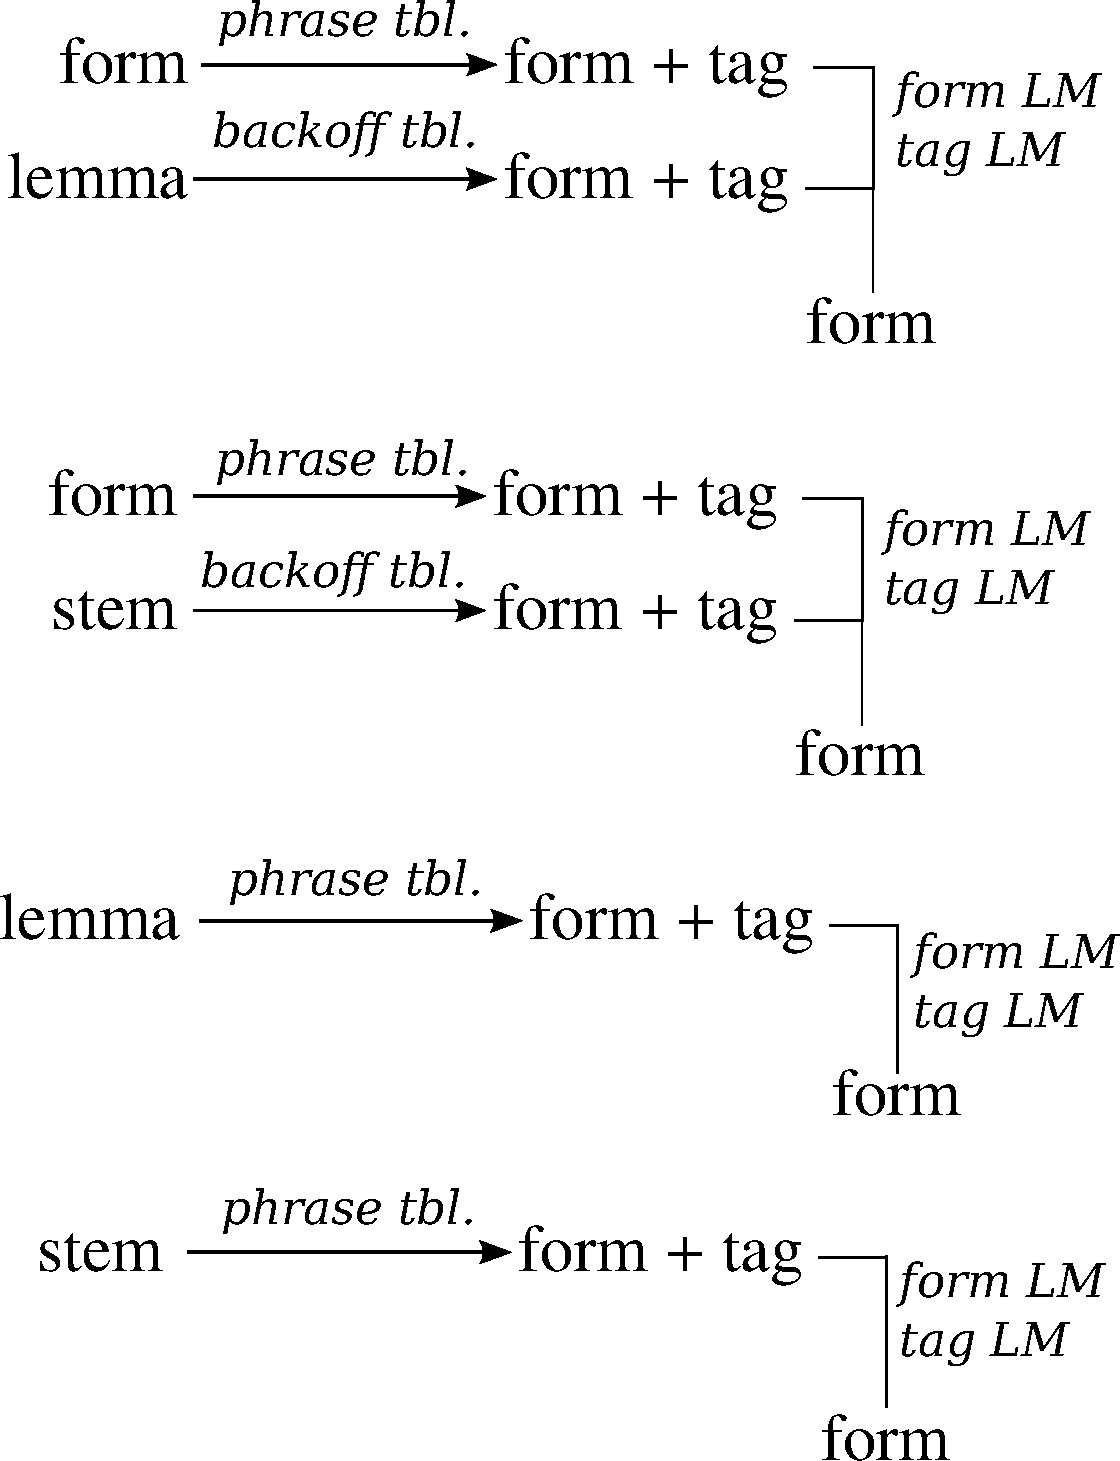
\includegraphics[width=0.4\textwidth]{graf_moses}
\caption{Factored set-up (various versions)}
\label{graf:mss}
\end{figure}

The whole factored set-up can be seen in the Figure~\ref{graf:mss}.

\subsection{Lemmatization, tagging}

%One of the ways to improve the out-of-vocabulary rate is using additional morphological
%information, the method that was successfully implemented for example by \cite{turchi},
%bringing a decrease of a OOV words without introducing more parallel data.

%Ja si nejsem jisty, jestli to, co delal Turchi je totez, co delame my.

We are exploiting the morphological features in two ways. First, we use lemmatization of source language (in this case, Russian) for making OOV rates smaller. Also, we use tagging of the target languages for better language models.

For Czech and English, we used Morče\footnote{\texttt{http://ufal.mff.cuni.cz/morce/}} - morphological perceptron-based tagger, developed at Charles' University in Prague. For Russian, we used TreeTagger\footnote{\texttt{http://www.ims.uni-stuttgart.de/\-projekte/corplex/TreeTagger/}} - modular tagger, developed at University of Stuttgart, with the Russian parameter file developed by Serge Sharoff.

Because the Russian is always the source language in this case, the tagset is not relevant. For Czech, Morče uses Czech positional tagset\footnote{See \texttt{http://ufal.mff.cuni.cz/pdt/\-Mor\-pho\-logy\-\_\-and\-\_\-Tag\-ging\-/\-Doc/hmptagqr.html}}. For English, Morče uses tagset derived from Penn Treebank.

\subsection{"Brute force" stemming}
In general, stemming is deriving a stem (root) for a word form in languages, where it makes sense.

In Slavic languages the inflection is done on the end of the word, so the stem is usually some beginning of the word form, unchanged.

There are some stemmers for all three languages that are trying to do this "properly". However, in our case, what we mean by stemming is just taking first $n$ letters of each word, with varying $n$ from 3 to 6 for different experiments.

We can argue that this stemming is really just "brute force" and should not give any good results. Surprisingly, the results are actually better than with the lemmatization.

%Karel: tohle je divne napsane, mazu to
%exploiting a stem(root) of a word is a primitive thus efficient technique to support OOV words guessing.
%Especially for the agglutinative languages stemming can bring some fruit because
%each morphemic category is related one-to-one to its surface form%(is it really so??)
%Czech and Russian are flective languages, so they combine the morphemes by fusion/flexion,
%not just putting it one after another. So for instance, if a substantive in Czech has categories
% number, gender and case, the morphemes presenting those categories will be represented only
%by one morpheme-ending. 
%As we tried to use the maximum of baseline data, we decided to derive stems from the words
%without using any additional morphological information like the list of word endlings that are to be eliminated.
%The technique is primitive - it presents taking the first n characters of a word and then selecting the optimal
%length of a stem that bring the better improvement of a Bleu score and OOV rate.
%The example of a stemmed text:\\
%En: \textit{the$|$the gaza$|$gaza cease$|$cease -$|$- fire$|$fire should$|$shoul be$|$be allowed$|$allow to$|$to facilitate$|$facil 
%reconciliation$|$recon between$|$betwe fatah$|$fatah and$|$and hamas$|$hamas}
%%We first tested it for Russian-to-Czech translation.
%The setup of this experiment is the same as the previous - factored, where stems are used instead of lemmas,
%the results are shown in Table \ref{tab:stem}.



%First we opted for taggers that are available  on-line. Those taggers
%(Morce for Czech, TreeTagger for Russian and English) assigned each word form with
%a lemma and a tag. 

%???????? opravdu??? je blbost jenom snizovat OOV.... 

%As our main task on the current stage was only to check
%how much words will be translated properly, we are more interested in increasing
%the OOV rate than a BLEU score. The latter is not supposed to be that 
%good for the evaluating translation into morphologically rich languages that often have
%free word order. Still, it will serves the purpose of comparison the translation 
%quality into the same language (we have chosen Czech as a target) under the same conditions(training data).

\section{Statistical Machine Translation setup}
%Statistical Machine Translation nowadays has become one of the easiest and cheapest paradigms of the MT systems. 
%To jsou proste vyplnove reci, mam pocit...
%Researchers can now usevarious toolkits to experiment with different language pairs.

\subsection{Moses}
From the various available tools, we chose to experiment with Moses, an open-source implementation of phrase-based statistical translation system.

%\subsection{Moses}
The Moses toolkit \cite{moses} is a complex system which includes many components
for data preprocessing and MT evaluation, for example
GIZA++ %\footnote{http://www.fjoch.com/GIZA++.html}
involved in finding word alignment, the SRI Language Modeling
Toolkit %\footnote{http://www.speech.sri.com/projects/srilm/} 
and the built-in implementation of model optimization (Minimum Error Rate Training, MERT) on a
given development set of sentences.
%We included direct translation as a basic setting.
%There are still weights
%combining phrase and language model into a log-linear model to be mentioned.
%They are tuned by Minimum error rate training (MERT) algorithm which is driven
%by BLEU feedback scored on held-out sentences.


Factors have been described in the section above.

\subsection{Data}
%Phrase-based SMT systems need huge amount of parallel data in order to
%extract dictionaries of phrases and their translations, so called phrase tables.
\begin{table}

\begin{center}
\begin{tabular}{lcr}
  &  Languages & Sentences \\
\hline
%Language Model & cs & 92,233 \\
%Language Model & en & 92,233 \\
Train & ru $\rightarrow$ cs &  93395\\
Train & ru $\rightarrow$ en &  92775\\ \hline %TODO ru-en
Dev & cs, en, ru          &    765 \\
Test  & cs, en, ru          &  2000 \\
\hline
\end{tabular}
\end{center}
\caption{Parallel corpus size.}
\label{tab:corpus}
\end{table}

In our experiment we exploited data from a parallel Czech-English-Russian
corpus called UMC (UFAL Multilingual Corpus) with automatic pairwise sentence
alignment. The texts were downloaded from the Project
Syndicate\footnote{http://www.project-syndicate.org/} page. 
The data are divided into three sets: training set (train),
development set (dev) for MERT and test set for testing BLEU and OOV rates.
The statistics of the data are summarized in the Table \ref{tab:corpus}.

As we can see, the number of sentences is slightly different for different language pairs; it is because the sentences are not always aligned one-to-one, but often one-to-many, many-to-many or zero-to-many. We decided to take all of the sentences, where the alignment is non-zero on one end. 

\section{Results}
%TURESULTS

We use the following convention in this section: the baseline result is just called "baseline". Baseline doesn't use any tagging, stemming or lemmatizing; it is "only" run with the basic Moses setting.

The versions with only stem or lemma on the source side are marked with "1-" at the beginning and the versions with both form and lemma on the source side are marked with "2-" (as in "1 phrase table" or "2 phrase tables").

The various version are then named according to the technique of decreasing OOV - that is, "-stem3" with stem, "-lemma" with lemmatization.

So, for example, "2-lemma" means the version with lemmatization and two phrase tables.

\subsection{Russian to Czech}

\begin{figure}
\centering
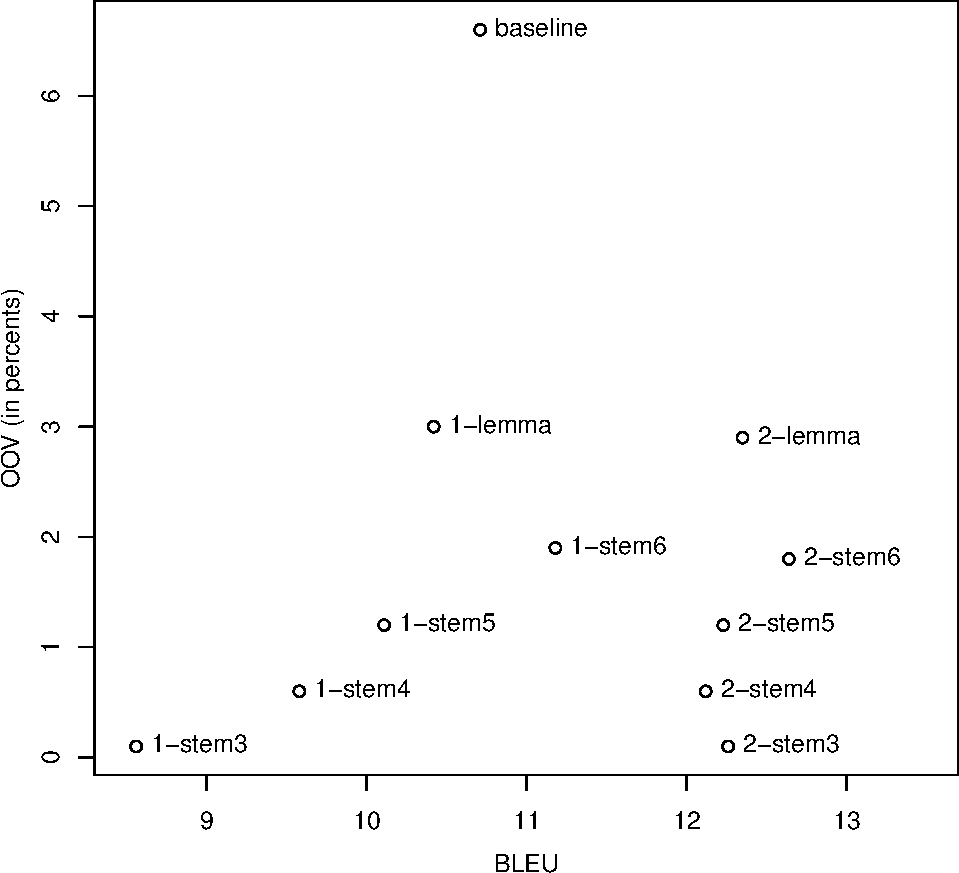
\includegraphics[width=0.5\textwidth]{plot_csru}
\caption{Russian to Czech results}
\label{graf:csru}
\end{figure}

\begin{table}

\begin{center}
\begin{tabular}{|r|l|l|}
  \hline
  \textbf{Type} & \textbf{OOV} & \textbf{BLEU} \\
\hline
baseline & 6.65 &  10.71 ($\pm$ 0.56) \\ \hline %s.evaluatorcyrillics.bbc23901.20130205-1730
1-lemma & 3.03  & 10.42($\pm$ 0.57) \\ \hline   %s.evaluatorcyrillics.99ee3eec.20130205-1850
1-stem3 & 0.16 & 8.56($\pm$ 0.53) \\ \hline     %s.evaluatorcyrillics.b3ffaca7.20130205-1849
1-stem4 & 0.67 & 9.58($\pm$ 0.50)\\ \hline      %s.evaluatorcyrillics.8674fd52.20130205-1848
1-stem5 & 1.21 & 10.11($\pm$ 0.57) \\ \hline    %s.evaluatorcyrillics.87f079da.20130205-1847
1-stem6 & 1.91 & 11.18($\pm$ 0.55)\\ \hline     %s.evaluatorcyrillics.fd9a46a5.20130205-1846
2-lemma & 2.92 & 12.35($\pm$ 0.58) \\ \hline    %s.evaluatorcyrillics.0b217d47.20130205-2256
2-stem3 & 0.17 & 12.26($\pm$ 0.64) \\ \hline    %s.evaluatorcyrillics.abee4dcc.20130205-1915
2-stem4 & 0.67 & 12.12($\pm$ 0.58) \\ \hline    %s.evaluatorcyrillics.9b929690.20130205-1914
2-stem5 & 1.22 & 12.23($\pm$ 0.59) \\ \hline    %s.evaluatorcyrillics.99998a35.20130205-1913
2-stem6 & 1.88 & 12.64($\pm$ 0.60) \\           %s.evaluatorcyrillics.c0cd4c8c.20130205-1909

\hline
\end{tabular}
\end{center}
\caption{Results for Russian-to-Czech}
\label{tab:rescs}
\end{table}

The results for Russian to Czech translation are in the Figure \ref{graf:csru} and in Table \ref{tab:rescs} (with the 95\% confidence intervals with BLEU). As we can see, 1-stem3 decreased OOV to nearly zero, but the BLEU went down, too. We can also see that the adding of phrase table from form as the main table makes the results better overall.

What was surprising to us is that "brute force" stemming can actually achieve better OOV rate \textbf{and} BLEU score (although the differences in BLEU score are inside the confidence interval).

We can see that we can both decrease the OOV and increase the BLEU score.

\subsection{Russian to English}

\begin{figure}
\centering
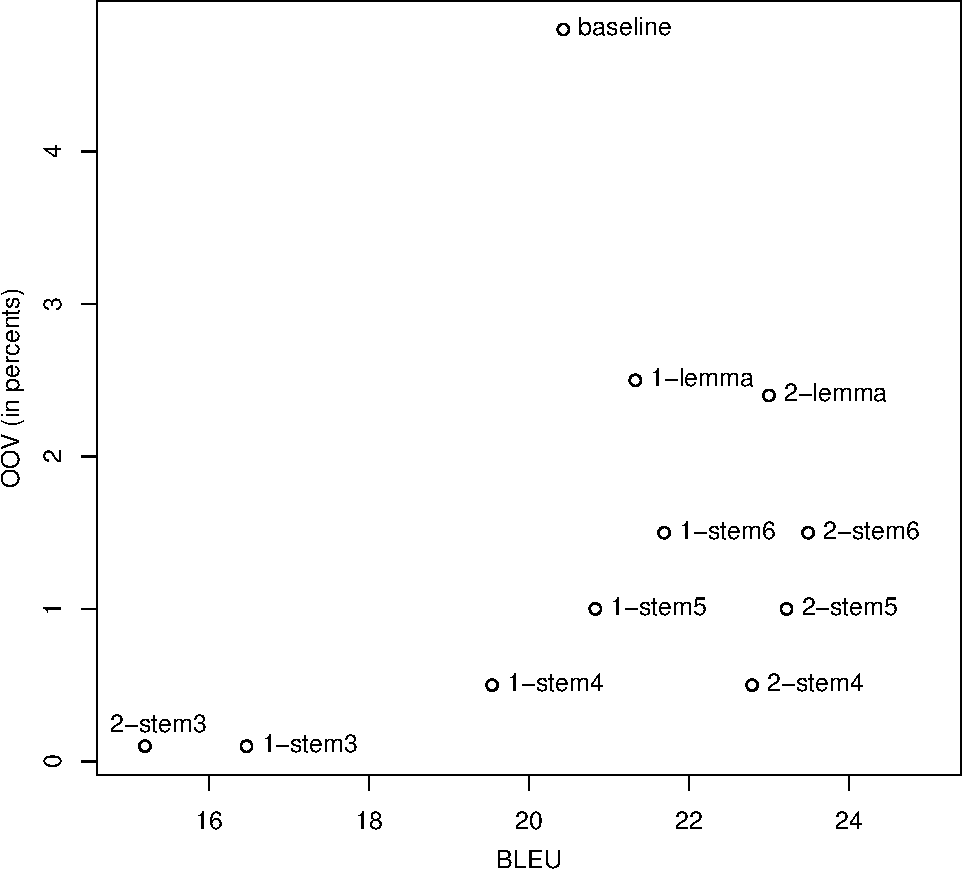
\includegraphics[width=0.5\textwidth]{plot_enru}
\caption{Russian to English results}
\label{graf:enru}
\end{figure}

\begin{table}

\begin{center}
\begin{tabular}{|r|l|l|}
  \hline
  \textbf{Type} & \textbf{OOV} & \textbf{BLEU} \\
\hline



baseline & 4.81 & 20.43($\pm$ 0.71) \\ \hline %s.evaluatorcyrillics.8032ce6d.20130205-2236
1-lemma & 2.56 & 21.33($\pm$ 0.73) \\ \hline %s.evaluatorcyrillics.fa1910b0.20130205-2350
1-stem3 & 0.11 & 16.47($\pm$ 0.60) \\ \hline %s.evaluatorcyrillics.74f57dd5.20130205-2349
1-stem4 & 0.51 & 19.54($\pm$ 0.69) \\ \hline %s.evaluatorcyrillics.af956c9a.20130205-2346
1-stem5 & 1 & 20.83($\pm$ 0.74) \\ \hline %s.evaluatorcyrillics.f1600b72.20130205-2246
1-stem6 & 1.53 & 21.69($\pm$ 0.71) \\ \hline %s.evaluatorcyrillics.8b125510.20130205-2352
2-lemma & 2.45 & 23($\pm$ 0.79) \\ \hline %s.evaluatorcyrillics.8f7db9fa.20130205-2248
2-stem3 & 0.12 & 15.2($\pm$ 0.76) \\ \hline %s.evaluatorcyrillics.6df7e7ab.20130205-2249
2-stem4 & 0.5 & 22.79($\pm$ 0.77) \\ \hline %s.evaluatorcyrillics.c030f500.20130205-2344
2-stem5 & 1 & 23.22($\pm$ 0.79) \\ \hline %s.evaluatorcyrillics.5495eca7.20130205-2252
2-stem6 & 1.52 & 23.49($\pm$ 0.79) \\ %s.evaluatorcyrillics.6b052d73.20130205-2347

\hline
\end{tabular}
\end{center}
\caption{Results for Russian-to-English}
\label{tab:resen}
\end{table}
The results for Russian to English translation are in the Figure \ref{graf:enru} and in Table \ref{tab:resen} (with the 95\% confidence intervals with BLEU).

We can again see the same general trends as in previous example - but it's not that surprising, taking into consideration the fact that the source text is the same. Again, brute-force stemmers work better than lemmatizers. (There is something unusual in 1-stem3 and 2-stem3, where 2-stem3 BLEU is unexpectedly lower, than 1-stem3. Given that the translations from 3 lettered stem are not very truststworthy, we consider this just a strange anomaly.)

What is, however, surprising is, that the "deeper" relationship between Russian and Czech \textbf{doesn't help the translation at all}. The BLEU score is higher in Russian to English, the OOV rate too. Again, as we touched upon this issue before, this is probably mainly the fault of the morphological richness of Slavic languages. 

Even though, the results were still a little unexpected to us. 

A small note: with experience from our past experiments, we think, that if we chose to do the experiments in the other direction - from Russian to English, the results would be less promising, as it is generally translation \textbf{into} 
a morphologically rich language that causes problems.
%nejsem si jistej, jestli je to pravda.... ale neověřim to, protože nám právě došlo místo na ufallabu.

\section{Conclusion}
In this paper we have shown two ways to improve the translation quality and lower out-of-vocabulary rate: with the help of lemmatizing and stemming. 


We have shown that surprisingly, "brute force" stemming works better for both BLEU and OOV rates, than lemmatization, and that ideal length is six letters. 

We have also shown that morphological closeness of two rich languages is not helping us in SMT, if we have the same amount of parallel data.



%These models have shown an improvement in terms of BLEU
%score and a considerable decrease of out-of-vocabulary words, especially for the morphologically rich languages. 

%The OOV rate for the translation between Czech and Russian reduced 2 times(lemma model) and 5 times(stem model) 
%against the baseline. The improvement in terms of OOV for English-Czech translation was not
%significant and the BLEU score has not changed a lot as well.
%Our future plans are to exploit more data
%and this improvement was even more significant than for the respective rate for English-to-Czech translation. 


\begin{thebibliography}{} 

%--\bibitem{baltic} Raivis Skadin¹, Karlis Goba, and Valters ©ics: Improving SMT for Baltic Languages with Factored Models. 
%--In: Proceedings of the 2010 conference on Human Language Technologies, 125-132, 2010.

\bibitem[Habash 2008]{habash} Habash, N.: Four techniques for online handling of out-of-vocabulary words in 
Arabic-English statistical machine translation. In: Proceedings of the 46th Annual Meeting of 
the Association for Computational Linguistics on Human Language Technologies:
%----Short Papers (HLT-Short '08). Association for Computational Linguistics, 
Stroudsburg 2008, PA, USA, 57-60.
%???2008???nevim

\bibitem[Popovic and Ney 2004]{popovic} Popovic,M., Ney, H.: Towards the Use of Word Stems and Suffixes for Statistical Machine Translation. 
In: Proceedings of 4th International Conference on Language Resources and Evaluation (LREC), Lisbon, Portugal, May 2004 

\bibitem[Oflazer 2008]{oflazer} Oflazer, K.:Statistical Machine Translation into a Morphologically Complex Language. 
In: Proceedings of CICLing 2008, Haifa, Israel, February 17-23, 2008. 

\bibitem[Gispert et al. 2005]{gispert} Gispert,A., Marino,J, Crego, J: Improving statistical machine translation by classifying and generalizing inflected verb forms.  
In: Proceedings of 9th European Conference on Speech Communication and Technology. 2005.

\bibitem[Turchi et al. 2011]{turchi} Turchi, M., Ehrmann, M.: Knowledge Expansion of a Statistical Machine Translation System using Morphological Resources. 
In: Polibits, (43), 37-43, 2011.

\bibitem[Bojar and Tamchyna 2011]{bojartamchyna} Bojar,O., Tamchyna, A.: Forms Wanted: Training SMT on Monolingual Data.
In: Proceedings Research Workshop of the Israel Science Foundation University of Haifa, Israel. 2011.

\bibitem[Koehn et al. 2007]{moses}Koehn, P., H. Hoang, A. Birch et al: Moses: Open source toolkit for statistical machine translation.
In: Proceeding ACL '07 Proceedings of the 45th Annual Meeting of the ACL, pp. 177-180, ACL, 2007.

\end{thebibliography}


\end{document}

